\documentclass[10pt,letterpaper]{article}
\usepackage[margin=0.7in,headheight=14pt,headsep=16pt,footskip=24pt]{geometry}
\usepackage[T1]{fontenc}
\usepackage{lmodern,microtype,graphicx,booktabs,amsmath,array,enumitem}
\usepackage[dvipsnames]{xcolor}
\usepackage{caption,fancyhdr,titlesec,tikz,listings}
\usetikzlibrary{arrows.meta,positioning}
\usepackage[colorlinks=true,linkcolor=MidnightBlue,urlcolor=MidnightBlue,citecolor=MidnightBlue]{hyperref}
\definecolor{accent}{HTML}{195875}
\definecolor{pale}{HTML}{EEF4F7}
\pagestyle{fancy}
\fancyhf{}
\fancyhead[L]{\small CSE498 \quad Object Detection Project}
\fancyhead[R]{\small YOLO11 / YOLOE}
\fancyfoot[C]{\small \thepage\ / 6}
\renewcommand{\headrulewidth}{0.3pt}
\setlength{\parindent}{0pt}
\setlength{\parskip}{4pt}
\setlength{\textfloatsep}{10pt}
\captionsetup{font=small,labelfont=bf,skip=5pt}
\titleformat{\section}{\large\bfseries\color{accent}}{\thesection.}{0.5em}{}
\titleformat{\subsection}{\normalsize\bfseries}{\thesubsection}{0.5em}{}
\titlespacing*{\section}{0pt}{4pt}{7pt}
\titlespacing*{\subsection}{0pt}{7pt}{3pt}
\setlist[itemize]{leftmargin=16pt,itemsep=2pt,topsep=3pt}
\lstset{basicstyle=\ttfamily\small,backgroundcolor=\color{pale},frame=single,
  rulecolor=\color{pale},columns=fullflexible,breaklines=true,showstringspaces=false,
  aboveskip=6pt,belowskip=6pt,xleftmargin=4pt,xrightmargin=4pt}
\newcommand{\takeaway}[1]{\par\noindent\colorbox{pale}{\parbox{\dimexpr\linewidth-2\fboxsep}{\small\textbf{Main point.} #1}}\par}
\newcommand{\fig}[3]{\begin{center}\includegraphics[width=#2\linewidth]{figures/#1}\captionof{figure}{#3}\end{center}}
\begin{document}

{\LARGE\bfseries YOLO11 and Open-Vocabulary Detection\\[2pt] in Apartment Images\par}
{\small GitHub: \texttt{lllingshen} \hfill September 6, 2026}\par
{\small Repository: \url{https://github.com/lllingshen/CSE498}}

\textbf{Overview.} I tested pretrained YOLO11 on two apartment photographs, fine-tuned a bottle detector with a small labeled dataset, and used text-prompted YOLOE to request additional object categories. Increasing model capacity and image size recovered useful detections. Bottle fine-tuning improved a small validation score but produced many false positives in the apartment. YOLOE added some useful labels outside COCO, although it still made mistakes. This report explains both the methods and these limitations.

\section{How YOLO11 works}
YOLO11 is a one-stage detector: one network predicts object locations and class scores from an image, without a separate region-proposal stage. I began with the assigned webcam repository~\cite{upstream}, whose \texttt{main.py} reads a camera frame, calls YOLO, and draws boxes. My image experiment replaces the camera loop with two saved JPG files. The existing repository files were preserved.

\begin{center}
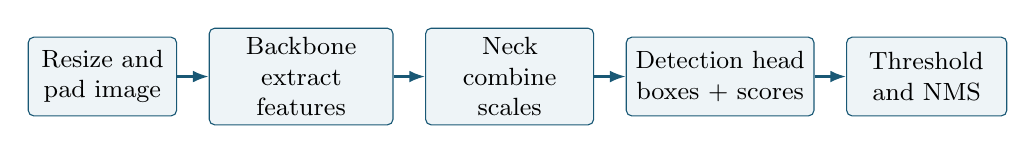
\begin{tikzpicture}[node distance=4mm,box/.style={draw=accent,fill=pale,rounded corners=2pt,minimum height=10mm,align=center,font=\small},arr/.style={-{Latex[length=2mm]},thick,draw=accent}]
\node[box,text width=1.65cm] (in) {Resize and\\pad image};
\node[box,text width=2.1cm,right=of in] (back) {Backbone\\extract features};
\node[box,text width=1.9cm,right=of back] (neck) {Neck\\combine scales};
\node[box,text width=2.15cm,right=of neck] (head) {Detection head\\boxes + scores};
\node[box,text width=1.8cm,right=of head] (out) {Threshold\\and NMS};
\draw[arr] (in)--(back);\draw[arr] (back)--(neck);\draw[arr] (neck)--(head);\draw[arr] (head)--(out);
\end{tikzpicture}
\captionof{figure}{Simplified detection flow, drawn from the YOLO11 implementation~\cite{implementation}.}
\end{center}

\textbf{Backbone and neck.} The backbone reduces spatial resolution while learning increasingly useful visual features. C3k2 blocks process and recombine convolutional features. SPPF uses sequential pooling to collect wider context, while C2PSA applies attention to a feature branch. The neck combines fine and coarse features through upsampling, concatenation, and downsampling. This helps the detector handle objects at different sizes. The head reads three feature scales with strides 8, 16, and 32~\cite{implementation}.

\textbf{Head and training.} Separate branches predict box geometry and class scores. The implementation is anchor-free with respect to predefined box shapes: distances are predicted from feature-grid points. Each box side uses a 16-bin distribution, which is decoded into a distance. Training combines box overlap/localization loss (CIoU), classification loss (binary cross-entropy), and distribution focal loss (DFL). The matching procedure assigns suitable predictions to labeled objects. These operations let the model learn both \emph{where} an object is and \emph{what} it is~\cite{implementation}.

\textbf{Inference.} The confidence threshold removes low-scoring predictions. Non-maximum suppression (NMS) suppresses overlapping, lower-scoring boxes. Its overlap measure is
\[
\operatorname{IoU}(A,B)=\frac{|A\cap B|}{|A\cup B|}.
\]
The pretrained weights use 80 COCO categories~\cite{yolo11}. Changing a threshold cannot add a missing category such as a computer tower. A confidence score is a model prediction score, not the measured accuracy of the whole system.

\newpage
\section{Experiment 1: pretrained detection on my apartment}
I used two existing apartment photographs: a desk area and a kitchen. Each image is $8192\times5464$ pixels. This run did not capture new webcam images. The photos were retained unchanged, and inference used the full images; figure crops in this report only improve readability. I inspected the outputs qualitatively because there are no complete ground-truth boxes for these photographs.

\subsection{Starting from the repository settings}
The initial model was the repository's \texttt{yolo11n.pt}, with confidence 0.50 and image-size setting 640. It returned only two boxes in the desk photo and eight in the kitchen. One \texttt{tv} box covered both monitors, while the keyboard, mouse, phone, sink, and several smaller objects were missed. The actual padded input was $448\times640$, so the very large photographs lost substantial detail before reaching the network.

\subsection{A more useful pretrained configuration}
I compared larger input sizes and lower thresholds, then tried YOLO11m. The selected configuration used \texttt{imgsz=1920}, \texttt{conf=0.25}, and NMS IoU 0.45 with class-agnostic suppression. This last setting can suppress a phone that is predicted twice under different labels, although it can also suppress real, overlapping objects. The actual input was $1312\times1920$. This was parameter/model selection, \textbf{not fine-tuning}: no weights were trained in Experiment 1.

\begin{center}
\begin{tabular}{lrrp{6.9cm}}
\toprule
Configuration & Desk & Kitchen & Qualitative observation \\
\midrule
YOLO11n, 640, 0.50 & 2 & 8 & Sparse output; both monitors merged. \\
YOLO11m, 1920, 0.25 & 7 & 24 & Monitors separated; keyboard, mouse, phone, sink, banana, and more containers found. \\
\bottomrule
\end{tabular}
\captionof{table}{Prediction counts, not counts of verified correct objects. Model size, resolution, threshold, and NMS settings changed together.}
\end{center}

\fig{closed_set_detail.png}{1}{Selected monitor and input-device predictions, shown in a desk crop. The source CSVs retain every prediction from the full-image runs.}

The improved output was still imperfect. The dishwasher was labeled \texttt{oven}, some cabinet bottle boxes remained ambiguous, and the chair box did not cover its entire extent. YOLO11's COCO label \texttt{tv} was used for the computer displays; it is not a separate monitor class. Objects such as headphones, a digital piano, and a rice cooker do not have exact categories in this pretrained vocabulary.

\takeaway{More image detail and a stronger pretrained model helped recover visible objects. However, more boxes alone do not demonstrate higher accuracy, and these trials do not isolate the effect of each changed parameter.}

\newpage
\section{Experiment 2: fine-tuning with 50 bottle images}
\subsection{Dataset choice and split}
I selected bottles because the white insulated bottle on the desk was missed and some kitchen bottle predictions were weak or poorly localized. I first checked RefCOCO. It includes bottle instances, but is organized around referring expressions over COCO images~\cite{refcoco}. A detection conversion must include all relevant instances in an image, not only the one named by an expression. Since the starting YOLO11 weights were already COCO-pretrained, I used Open Images bounding-box data for a simpler small detection dataset~\cite{openimages}.

The dataset contains exactly \textbf{50 distinct images and 81 bottle boxes}. From the Open Images official validation pool, I excluded images with bottle group or depiction annotations, shuffled eligible image IDs with seed 42, and selected 50. The first 40 became the course training split (66 boxes); the remaining 10 became validation (15 boxes). This is a custom split, not the official Open Images train/validation division. Image IDs and image hashes are disjoint, and a perceptual-hash check found no near-duplicate candidates. The apartment photos were not included.

For each image, all provided bottle boxes were converted to YOLO format: class ID, normalized center coordinates, width, and height. This subset mainly contains drink, wine, and cosmetic bottles, not apartment scenes or insulated bottles specifically. Some source labels appear noisy; these were retained and documented. Image authors, source links, licenses, and hashes are included in the dataset manifest.

\subsection{Training setup}
Following the assigned fine-tuning workflow~\cite{finetutorial}, I loaded the same YOLO11m base model and changed the task to a single class, \texttt{bottle}. The first ten top-level modules' parameters were frozen, and other trainable layers were fine-tuned. This does not freeze the entire backbone. It is ordinary partial fine-tuning; \textbf{LoRA was not used or required by the supplied instructions}.

\begin{lstlisting}[language=Python]
model = YOLO("yolo11m.pt")
model.train(data="data.yaml", epochs=30, patience=10,
            imgsz=960, batch=4, freeze=10,
            optimizer="AdamW", lr0=0.0005,
            seed=42, device=0, workers=0, amp=False)
\end{lstlisting}

Training ran on an RTX 5090 using Ultralytics 8.4.142 and PyTorch 2.7.1+cu128. It stopped after \textbf{17 epochs}, with the best checkpoint from \textbf{epoch 7}. The maximum was 30 epochs, but patience 10 stopped training after ten epochs without a better validation result. The checkpoint is included for demonstration without retraining.

\fig{training_curves.png}{1}{Recorded training curves. The dashed line marks epoch 7. These internal validation curves use the training run's NMS IoU 0.7; the final before/after evaluation uses 0.45 for both models.}

\takeaway{Fine-tuning really updated network weights. Freezing some layers is different from LoRA, which would introduce trainable low-rank weight updates. The small dataset makes it especially important to check behavior outside the validation images.}

\newpage
\section{What I learned from fine-tuning}
\subsection{A fair bottle-only comparison}
I evaluated the pretrained and fine-tuned models on the same ten validation images. Both used CPU inference, image size 960, confidence 0.001, and NMS IoU 0.45. The low confidence threshold retains predictions across the precision--recall curve used for AP. The original COCO bottle class is ID 39; the fine-tuned dataset uses ID 0. The evaluation code selects bottle scores and maps the class ID consistently before NMS and matching.

\begin{center}
\begin{tabular}{lrr}
\toprule
Validation metric (10 images, 15 labeled bottles) & Before & After \\
\midrule
AP50 & 0.7630 & 0.9290 \\
AP50--95 & 0.5586 & 0.6052 \\
\bottomrule
\end{tabular}
\captionof{table}{Measured bottle AP on the fixed validation split. These images also selected the best checkpoint, so this is not an independent test score.}
\end{center}

AP50 measures detection performance with an IoU matching threshold of 0.50; AP50--95 averages over stricter thresholds from 0.50 to 0.95. Since the evaluation has one class, its AP is also the single-class mAP. The increase indicates better performance on these labeled validation images, not proof of a general improvement.

\subsection{The apartment results tell a different story}
The apartment comparison used the same image size 1920, confidence 0.25, and NMS IoU 0.45 before and after training. Only bottle predictions were compared. The desk count increased from 1 to 12, and the kitchen count from 15 to 26. These increases were largely misleading: many additional boxes were false positives or duplicate parts of a real bottle.

\fig{fine_tuning_examples.png}{1}{Selected post-training predictions. The white bottle is a plausible new detection, but the chair and stove are clearly not bottles. Colors indicate qualitative review of these examples, not a complete ground-truth evaluation.}

The fine-tuned model newly detected the white insulated bottle, but also called monitors, the computer tower, chair parts, a shopping bag, and a glass-covered appliance \texttt{bottle}. In the kitchen, false bottle labels appeared on the microwave, cabinet door, stove, and kettle. Some incorrect scores exceeded 0.95. Confidence was therefore not a reliable guarantee of correctness.

\subsection{Interpretation and limitations}
The specialist did not reliably improve my apartment photos and should not replace the general 80-class model. A small mostly positive, object-focused dataset, scene differences, single-class adaptation, and label noise are plausible contributors. This experiment does not separate their effects. The 10-image validation set is small and was reused for model selection; it cannot establish generalization to cluttered rooms.

For a stronger follow-up, I would collect more training-like indoor scenes, review ambiguous annotations, include useful background examples, and reserve a separate test set before adjusting settings. I would also evaluate false positives and recall against manual boxes. I did not alter this dataset or retrain repeatedly to hide the observed failure.

\takeaway{A higher validation AP and a larger number of boxes can coexist with worse behavior in a new scene. Testing the actual intended use case is essential.}

\newpage
\section{Open-set detection and the YOLOE architecture}
\subsection{From fixed classes to requested categories}
A closed-set detector is trained to output a fixed list of categories. In this project, ordinary pretrained YOLO11 used the 80 COCO labels. Open-set detection addresses objects beyond a fixed known label set; open-vocabulary methods often make this practical by accepting category names as text. My experiment is specifically \textbf{text-prompted open-vocabulary detection}, corresponding to the assignment's open-set task. It does not test a system that discovers and reliably names every unknown object automatically.

YOLOE keeps YOLO-style multi-scale image features and localization while making recognition depend on prompt embeddings~\cite{yoloepaper,yoloedocs}. Rather than having only a fixed class-score channel for each COCO category, its recognition branch compares region features with representations of requested classes. It also supports instance masks, although I only displayed and inspected boxes.

\begin{center}
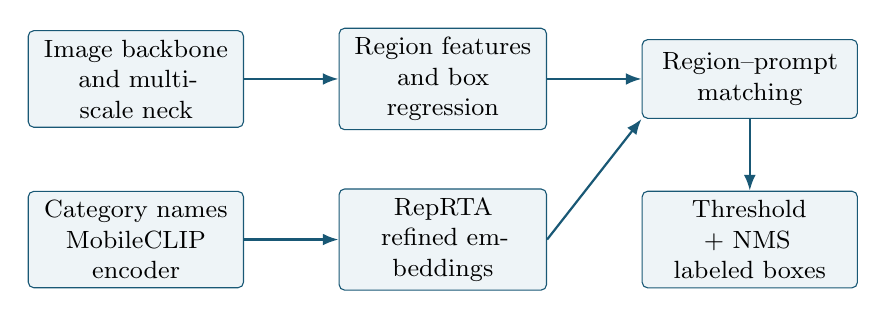
\begin{tikzpicture}[node distance=7mm,box/.style={draw=accent,fill=pale,rounded corners=2pt,align=center,font=\small,minimum height=10mm},arr/.style={-{Latex[length=2mm]},thick,draw=accent}]
\node[box,text width=2.5cm] (image) {Image backbone\\and multi-scale neck};
\node[box,text width=2.4cm,right=12mm of image] (region) {Region features\\and box regression};
\node[box,text width=2.5cm,right=12mm of region] (score) {Region--prompt\\matching};
\node[box,text width=2.5cm,below=8mm of image] (words) {Category names\\MobileCLIP encoder};
\node[box,text width=2.4cm,right=12mm of words] (reprta) {RepRTA\\refined embeddings};
\node[box,text width=2.5cm,right=12mm of reprta] (output) {Threshold + NMS\\labeled boxes};
\draw[arr] (image)--(region);\draw[arr] (region)--(score);\draw[arr] (words)--(reprta);
\draw[arr] (reprta.east)--(score.south west);\draw[arr] (score)--(output);
\end{tikzpicture}
\captionof{figure}{Conceptual text-prompt route used in this project. The diagram omits the mask branch and the unused visual/prompt-free routes.}
\end{center}

\textbf{RepRTA: Re-parameterizable Region-Text Alignment.} A text encoder provides embeddings for the names. A small learned auxiliary network refines them for region--text alignment. For a fixed vocabulary, the paper describes folding the refined embeddings into the classification convolution to reduce inference overhead. In my run, text embeddings were computed once and saved; I did not measure the paper's zero-overhead claim or execute the full fixed-classifier reparameterization~\cite{yoloepaper,yoloedocs}.

\textbf{SAVPE: Semantic-Activated Visual Prompt Encoder.} This is the visual-prompt alternative: semantic features are combined with an activation branch that weights positions associated with a selected image region. A user can point to an example object instead of supplying only a name. No visual prompt was supplied in this experiment~\cite{yoloepaper}.

\textbf{LRPC: Lazy Region-Prompt Contrast.} The prompt-free route uses a built-in vocabulary. It first selects likely object regions, then applies vocabulary matching to the retained locations, rather than evaluating a large vocabulary everywhere. This route does not require a generative language model. I did not run the prompt-free checkpoint~\cite{yoloepaper}.

These mechanisms are alternative ways to supply recognition information, not three steps that every YOLOE call must execute. Changing text prompts can request a new label without fine-tuning on these two photographs, but success still depends on what the pretrained representations can distinguish. Open vocabulary does not remove missed detections, category confusion, or false positives.

\newpage
\section{Experiment 3: text-prompted YOLOE and conclusions}
I followed the assigned text-prompt workflow~\cite{openTutorial}, using \texttt{get\_text\_pe}, \texttt{set\_classes}, and \texttt{predict}. The tutorial used YOLOE-v8l; my run used the supported \texttt{yoloe-11m-seg.pt} with MobileCLIP-B(LT). This is a workflow adaptation, not an exact reproduction of the tutorial's model and hardware. I selected 33 English category names after looking at the input scenes and fixed them before inspecting YOLOE output. Both photos used the same vocabulary, image size 1920, confidence 0.25, and NMS IoU 0.7 on CPU.

The model returned 24 desk boxes and 36 kitchen boxes. Useful examples included the computer tower (0.44), electric kettle (0.92), and faucet (0.95). However, the digital piano was labeled as a computer keyboard, the tissue box as a shopping bag, and the dishwasher as an oven. Headphones and the full rice cooker still lacked correct detections. The counts are not accuracy measurements, and the vocabulary/settings differ from Experiment 1.

\fig{open_vocabulary_examples.png}{1}{Selected YOLOE successes (green) and errors (red), redrawn from saved box coordinates. All original detections remain in the repository; no boxes were removed from the saved experiment results.}

\textbf{What the three experiments show.} A stronger pretrained configuration recovered useful detail. Small-dataset fine-tuning increased bottle AP on validation but failed to generalize reliably to the apartment. YOLOE expanded the labels I could request, while still confusing visible objects. None of these experiments proves that almost every object was correctly detected. The apartment comparisons are qualitative, with no complete box or mask ground truth.

\textbf{Reproduction and demonstration.} The repository contains all three experiment scripts, the 50-image dataset with attribution, the trained bottle checkpoint, saved results, and an English demonstration guide. New runs write to a separate \texttt{runs/} directory. Official pretrained weights are downloaded with hash checks. The YOLOE demo reuses the recorded 33-class prompt embeddings, avoiding another text-encoder download; changing the vocabulary requires recomputing them. The Overleaf ZIP includes this source and all four image assets. The separate Colab notebook is an unexecuted reproduction template; the results reported here were obtained locally.

\vspace{1pt}
\begingroup
\footnotesize
\setlength{\parskip}{0pt}
\begin{thebibliography}{9}
\setlength{\itemsep}{2pt}
\bibitem{upstream} V. Uberti. \emph{Webcam Object Recognition}. \href{https://github.com/valeriouberti/webcam-object-recognition}{GitHub repository}, commit \texttt{e1279fa}. Accessed Sept. 6, 2026.
\bibitem{yolo11} Ultralytics. \emph{YOLO11}. \href{https://docs.ultralytics.com/models/yolo11/}{Official documentation}. Accessed Sept. 6, 2026.
\bibitem{implementation} Ultralytics. \emph{Source code v8.4.142}: \href{https://github.com/ultralytics/ultralytics/blob/v8.4.142/ultralytics/cfg/models/11/yolo11.yaml}{YOLO11 graph}, \href{https://github.com/ultralytics/ultralytics/blob/v8.4.142/ultralytics/nn/modules/head.py}{detection heads}, and \href{https://github.com/ultralytics/ultralytics/blob/v8.4.142/ultralytics/utils/loss.py}{losses}.
\bibitem{finetutorial} Roboflow. \emph{Train YOLO11 on a Custom Dataset}. \href{https://github.com/roboflow-ai/notebooks/blob/main/notebooks/train-yolo11-object-detection-on-custom-dataset.ipynb}{Assigned notebook}.
\bibitem{refcoco} L. Yu et al. \emph{Referring Expression Datasets API}. \href{https://github.com/lichengunc/refer}{Author repository and dataset description}.
\bibitem{openimages} Google. \emph{Open Images V7}. \href{https://storage.googleapis.com/openimages/web/download_v7.html}{Official downloads}; \href{https://storage.googleapis.com/openimages/web/factsfigures_v7.html}{annotations and licenses}. Selected image attribution is in the repository manifest.
\bibitem{yoloepaper} A. Wang, L. Liu, H. Chen, Z. Lin, J. Han, and G. Ding. \emph{YOLOE: Real-Time Seeing Anything}. ICCV, 2025, pp. 24591--24602. \href{https://openaccess.thecvf.com/content/ICCV2025/html/Wang_YOLOE_Real-Time_Seeing_Anything_ICCV_2025_paper.html}{Published paper}.
\bibitem{yoloedocs} Ultralytics. \emph{YOLOE}. \href{https://docs.ultralytics.com/models/yoloe/}{Official documentation}; \href{https://github.com/THU-MIG/yoloe}{authors' implementation}.
\bibitem{openTutorial} Roboflow. \emph{Zero-Shot Detection and Segmentation with YOLOE}. \href{https://github.com/roboflow-ai/notebooks/blob/main/notebooks/zero-shot-object-detection-and-segmentation-with-yoloe.ipynb}{Assigned notebook}.
\end{thebibliography}
\endgroup
\end{document}
